% A Preliminary Literature Review which indicates: 
% (i) that you have studied the work of the major authors in your research field 
% (ii) that you are familiar with the major themes relevant to that subject area 
% (iii) what further investigations you intend to pursue as part of this dissertation. 
% You should bear in mind that you are reviewing the literature in order to develop sharper, 
% more insightful and focused research questions about your topic. 
% Therefore, your literature review should lead to and justify your research objectives and questions.

% continuar a partir de:
% /home/joenio/src/bibliografia/Papers/Replication of Controlled Experiments in Empirical Software Engineering - A Survey.pdf

\xchapter{Fundamentação teórica}
{Este capítulo apresenta conceitos necessários para a compreensão do trabalho.}
\label{fundamentacao}

\section{Software acadêmico}

% Anúncio em destaque no ACM DL: Reproducibility of Results in the ACM Digital Library 
% http://dl.acm.org/docs/reproducibility.cfm

% ciencia aberta e desenvolvimento sustentavel
% https://ocsdnet.org/open-and-collaborative-science-using-knowledge-as-a-pathway-to-sustainable-development/

Segundo \citeonline{hettrick_2014_14809} software acadêmico ({\it research
software}) é todo software usado para gerar, processar ou analisar resultados
de pesquisas com intenção de ser publicados (seja num jornal, revista,
conferência, monografia, livro ou tese). Software de pesquisa pode ser qualquer
coisa entre poucas linhas escritas por você mesmo, até mesmo um software
desenvolvido profissionalmente. Software que não gera, processa ou analisa
resultados - como por exemplo um editor de textos, ou o uso de navegadores web
- não são considerados softwares de pesquisa, segundo esta definição.

%%% Softwares acadêmicos são softwares desenvolvidos no decorrer de pesquisas
%%% científicas como parte de um estudo a ser publicado (seja num jornal, revista,
%%% conferência, monografia, livro ou tese), podem ser pequenos scripts contendo
%%% poucas linhas de código, protótipos, ou mesmo produtos de software completos
%%% que demonstram ou refletem os resultados de uma pesquisa, costumam ser
%%% utilizados para gerar, processar ou analisar resultados, mas podem ser para
%%% qualquer outro fim, basta que seja um dos artefatos gerado na pesquisa, será
%%% considerado software acadêmico.
%%% 
%%% Tais softwares podem ser encontrados na literatura pelo nome de {\it research
%%% tool} \cite{Portillo12}, {\it research-originated software} \cite{Kon2011},
%%% %{\it research software} \cite{hettrick_2014_14809} ou
%%% {\it academic software} \cite{allen2017engineering}, e costumam ser citados
%%% pelos seus autores como uma contribuição do estudo, seja principal ou
%%% secundária, alguns autores criam softwares acadêmicos como meio para atingir os
%%% resultados da pesquisa e não descrevem muito bem o software.
%%% 
%%% %, traduzido para software acadêmico para evitar o
%%% %termo {\it software de pesquisa}, a palavra {\it research} em português {\it
%%% %pesquisa} pode ser facilmente confundida com ferramentas ou sistemas de
%%% %pesquisa, como sites de pesquisa por exemplo,
%%% 
%%% % este artigo \cite{howison2016software} faz exatamento o mesmo estudo que estou fazendo!
%%% 
%%% Copiar e usar exatamente esta linha de pensamento e argumentos:
%%% Yet, the visibility of software in the scientific record is in
%%% question, leading to concerns, expressed in a series of
%%% National Science Foundation (NSF)- and National Institutes
%%% of Health–funded workshops, about the extent that scientists
%%% can understand and build upon existing scholarship (e.g.,
%%% Katz et al., 2014; Stewart, Almes, & Wheeler, 2010). In
%%% particular, the questionable visibility of software is linked to
%%% concerns that the software underlying science is of question-
%%% able quality. These quality concerns are not just technical,
%%% but extend to the appropriateness of software for wide
%%% sharing, and its ability to facilitate the codevelopment that
%%% would make efficient use of limited scholarly funding
%%% (Howison & Herbsleb, 2013; Katz et al., 2014).
%%% The link is two-fold: First, when software is not visible, it
%%% is often excluded from peer review; second, its lack of
%%% visibility, or the particular form of visibility, means that
%%% incentives to produce high-quality, widely shared, and code-
%%% veloped software may be lacking. A well-functioning system
%%% would assist not only the goals of understanding and trans-
%%% parency, but also the goals of aiding replication (Stodden
%%% et al., 2010), complementing the availability of publications
%%% such that “the second researcher will receive all the benefits
%%% of the first researcher’s hard work” (King, 1995, p. 445).
%%% The situation with software is broadly analogous (but not
%%% identical) to that of data in publications; indeed, all data are
%%% processed by software in some form (Borgman et al., 2012).
%%% Nonetheless, there are relevant differences. Accordingly, our
%%% inquiry into the visibility of software in scholarly commu-
%%% nication is complementary to recent interest in data citation.
%%% In sum, then, the relationship of software to the scholarly
%%% 
%%% 
%%% Como não existe ainda amadurecimento suficiente sobre como citar softwares e
%%% outros artefatos em pesquisas científicas, não temos um padrão de como fazê-lo,
%%% cada autor cita à sua maneira, muitas vezes ao longo do texto, outras em seções
%%% específicas sobre a implementação do software, nem semprem informam onde
%%% encontrar uma cópia do software, ou ainda nem sobre o modelo em que o software
%%% é distribuído, ou se é de alguma forma distribuído ao público.
%%% 
%%% Os softwares acadêmicos neste estudo serão aquelas citados pelo autor como
%%% contribuição do estudo, então toda vez que citarmos software acadêmico estamos
%%% falando de artefatos de software citados pelo autor como contribuição do estudo.

\section{Ciência aberta}

Over the past fifteen years the scholarly communications agenda
has progressed gradually. Currently we are experiencing a strong
tendency among all research stakeholders to engage with the
practice of OS. Lately, research funders require the sharing not
only of the research results they have funded, but also of the
procedures and data that are being generated during the research
conduct. Researchers, on the other side, are keen on observing
their research results being used for the improvement of the
society and are forced by their funders to demonstrate the impact
of their research. At the same time, higher academic institutions
aim to join the OS agenda as well, since they see the opportunity
of great economic benefits and savings. While OS is the possible
answer to all these factors, the stakeholders’ inability to
understand the requirements for the application of OS can be a
suspensory factor for the OS implementation and evolution.
The aim of the FOSTER project is to advance the stakeholders'
knowledge on the usefulness of OS and explain the technicalities,
strategies and best practices using which OS can be applied. As an
attempt to educate the largest number of researchers possible,
FOSTER has created an e-leanring portal, which contains quality
assured information relating to the topic and it is open to everyone
in the world. The platform contains two types of information:
learning material and online courses. The classification of these
two types is supported by an OS taxonomy, where related terms
are applied both in the portal's material and also in the courses.
With the use of the taxonomy, users are in the position to
understand the OS domain and the concepts around it.
The main goal of the FOSTER project, which is mainly achieved
through the portal functionalities, is not only to educate the
research stakeholders on OS, but also to build a community of
researchers, librarians, software developers, funders and research
administrators who are interested in OS in order to advance the
way research is being conducted and shared. In addition, FOSTER
attempts to provide tools to this community, such as re-usable
content for training and a platform for blended learning and e-
learning courses that the community could run. This OS
advancement is essential for the research promotion and,
consequently, for the benefit of the society as a whole
\cite{Nancy2015}.

Open Science may be practised both
for philosophical and pragmatic reasons. As the
resources produced by open projects are
potentially accessible to public audiences, Open
Science offers both a novel medium for public
access and involvement in the process of science
and an innovative method for real-time science
communication. Does such direct access clear
the stream of communication or muddy the
waters with unfocussed, unclear and unvetted
comment? This paper suggests that adopting an
Open Science approach allows the capture of an
authentic and clear record of research.
However, researchers acknowledge this involves
opening their work up to a different type of
scrutiny \cite{Grand2010}.

Open Science is an emerging approach to the conduct of science, technology and engineering
projects, in which information about the whole of an ongoing investigation is made available
on and through the Internet. Adopting an Open Science approach means the audience for the
research can extend beyond the researchers involved to other researchers and to members of
the public. Thus, Open Science has implications for engineering research, practice,
publishing and public engagement with engineering. This paper reviews the history and
evolution of the Open Science movement, includes some reflections on the related areas of
Open Access, peer-review and public engagement with science and engineering and discusses
data gathered from interviews. The analysis suggests that interviewees have concerns about
issues such as precedence and protection of original work and the time needed to integrate
open science practices into daily work. Successfully working in such collaborations is likely
to require not only common practical tools but also the development of shared language and
understanding between researchers and members of the public. Interviewees recognise the
value of Open Science in collaborative research and its innovative facility to sustain direct
public access to research outputs. It also has the potential to allow members of the public to
make real practical contributions to research \cite{Grand2010Open}.

This white paper was written as a contribution to the “Imagining
Tomorrow’s University: Rethinking scholarship, education, and institu-
tions for an open, networked era” workshop, a joint NIH/NSF-funded
event held 8–9 March 2017 in Rosemont, IL. In this paper, I present an
overview of what I consider open science, its importance, and how it
plays a role in my research agenda. I also discuss challenges faced in
pursuing research openness, and recommend changes to university
leaders to address these barriers \cite{niemeyer2017open}.

Open to All?  Case studies of openness in research
Since the early 1990s, the open access movement has promoted the concept of openness in relation
to scientific research. Focusing initially upon the records of science in the form of the text of articles
in scholarly journals, interest has broadened in the last decade to include a much wider range of
materials produced by researchers. At the same time, concepts of openness and access have also
developed to include various kinds of use, by machines as well as humans.
Academic bodies, including funders and groups of researchers, have set out statements in support
of various levels of openness in research. Such statements often focus upon two key dimensions:
what is made open, and how; and to whom is it made open, and under what conditions? This study
set out to consider the practice of six research groups from a range of disciplines in order to better
understand how principles of openness are translated into practice \cite{Nesta2010}.

\section{Reprodutibilidade}


The lack of replicability and reproducibility of scientific studies based on
computational methods has lead to serious mistakes in published scientific
findings, some of which have been discovered and publicized recently. Many
strategies are currently pursued to improve the situation. This article reports the
first conclusions from the ActivePapers project, whose goal is the development
and application of a computational platform that allows the publication of
computational research in a form that enables installation-free deployment,
encourages reuse, and permits the full integration of datasets and software into
the scientific record. The main finding is that these goals can be achieved with
existing technology, but that there is no straightforward way to adapt legacy
software to such a framework \cite{hinsen2014activepapers}

Reproducibility verification is essential to the practice of the scientific method.
Researchers report their findings, which are strengthened as other independent groups
in the scientific community share similar outcomes. In the many scientific fields
where software has become a fundamental tool for capturing and analyzing data, this
requirement of reproducibility implies that reliable and comprehensive software platforms
and tools should be made available to the scientific community. The tools will empower
them and the public to verify, through practice, the reproducibility of observations that
are reported in the scientific literature. Medical image analysis is one of the fields in
which the use of computational resources, both software and hardware, are an essential
platform for performing experimental work. In this arena, the introduction of the Insight
Toolkit (ITK) in 1999 has transformed the field and facilitates its progress by accelerating
the rate at which algorithmic implementations are developed, tested, disseminated and
improved. By building on the efficiency and quality of open source methodologies, ITK has
provided the medical image community with an effective platform on which to build a daily
workflow that incorporates the true scientific practices of reproducibility verification. This
article describes the multiple tools, methodologies, and practices that the ITK community
has adopted, refined, and followed during the past decade, in order to become one of the
research communities with the most modern reproducibility verification infrastructure. For
example, 207 contributors have created over 2400 unit tests that provide over 84% code
line test coverage. The Insight Journal, an open publication journal associated with the
toolkit, has seen over 360,000 publication downloads. The median normalized closeness
centrality, a measure of knowledge flow, resulting from the distributed peer code review
system was high, 0.46 \cite{McCormick2014}.

Linked Open Science—Communicating, Sharing and Evaluating
Data, Methods and Results for Executable Papers.
Linked Open Science is an approach to solve challenges of an executable paper. It is a combination of four “silver
bullets”: 1) publication of scientific data, metadata, results, and provenance information using Linked Data principles,
2) open source and web-based environments for executing, validating and exploring research, 3) Cloud Computing
for efficient and distributed computing, and 4) Creative Commons for the legal infrastructure. We will use a realistic
scientific research setting related to research on deforestation of the Brazilian Amazon rainforest to provide scenarios
to illustrate the application of Linked Open Science \cite{Kauppinen2011}.

Among empirical software engineering studies, those based on data re-
trieved from development repositories (such as those of source code management,
issue tracking or communication systems) are specially suitable for reproduction.
However their reproducibility status can vary a lot, from easy to almost impossible
to reproduce. This paper explores which elements can be considered to characterize
the reproducibility of a study in this area, and how they can be analyzed to better
understand the type of reproduction studies they enable or obstruct. One of the
main results of this exploration is the need of a systematic approach to asses the
reproducibility of a study, due to the complexity of the processes usually involved,
and the many details to be taken into account. To address this need, a methodology
for assessing the reproducibility of studies is also presented and discussed, as a tool to
help to raise awareness about research reproducibility in this field. The application
of the methodology in practice has shown how, even for papers aimed to be
reproducible, a systematic analysis raises important aspects that render reproduction
difficult or impossible. We also show how, by identifying elements and attributes
related to reproducibility, it can be better understood which kind of reproduction
can be done for a specific study, given the description of datasets, methodologies and
parameters it uses \cite{gonzalez2012reproducibility}.


Science rests on peer review and the wide-spread dissemination of
knowledge. Software engineering research will advance further and
faster if the sharing of data and tools were easier and more wide-
spread. Pragmatic concerns hinder the realization of this ideal: the
time and effort required and the risk of being scooped. We examine
the costs and benefits of facilitating sharing in our field in an effort
to help the community understand what problems exist and find
a solution. We examine how other fields, such as medicine and
physics, handle sharing, describe the value of sharing for replication
and innovation, and address practical concerns such as standards
and warehousing. To launch what we hope will become an ongoing
discussion of solutions in our community, we present some ways
forward that mitigate the risk of sharing — partial sharing, registry,
escrow, and market \cite{barr2010shoulders}.

Computer systems research spans sub-disciplines that in-
clude embedded and real-time systems, compilers, network-
ing, and operating systems. Our contention is that a number
of structural factors inhibit quality research. We highlight
some of the factors we have encountered in our work and ob-
served in published papers and propose solutions that could
both increase the productivity of researchers and the quality
of their output \cite{Vitek2011}.

At various machine learning conferences, at
various times, there have been discussions
arising from the inability to replicate the
experimental results published in a paper.
There seems to be a wide spread view that we
need to do something to address this prob-
lem, as it is essential to the advancement
of our field. The most compelling argument
would seem to be that reproducibility of ex-
perimental results is the hallmark of science.
Therefore, given that most of us regard ma-
chine learning as a scientific discipline, being
able to replicate experiments is paramount.
I want to challenge this view by separating
the notion of reproducibility, a generally de-
sirable property, from replicability, its poor
cousin. I claim there are important differ-
ences between the two. Reproducibility re-
quires changes; replicability avoids them. Al-
though reproducibility is desirable, I contend
that the impoverished version, replicability,
is one not worth having \cite{drummond2009replicability}.

Abstract—This paper is the result of reviewing all papers
published in the proceedings of the former International
Workshop on Mining Software Repositories (MSR) (2004-2006)
and now Working Conference on MSR (2007-2009). We have
analyzed the papers that contained any experimental analysis
of software projects for their potentiality of being replicated.
In this regard, three main issues have been addressed: i) the
public availability of the data used as case study, ii) the public
availability of the processed dataset used by researchers and iii)
the public availability of the tools and scripts. A total number of
171 papers have been analyzed from the six workshops/working
conferences up to date. Results show that MSR authors use
in general publicly available data sources, mainly from free
software repositories, but that the amount of publicly available
processed datasets is very low. Regarding tools and scripts, for
a majority of papers we have not been able to find any tool,
even for papers where the authors explicitly state that they have
built one. Lessons learned from the experience of reviewing the
whole MSR literature and some potential solutions to lower the
barriers of replicability are finally presented and discussed
\cite{robles2010replicating}.



Enquanto pesquisadores publicam artigos descrevendo e divulgando seus
resultados, é raro que façam o mesmo com toda a produção gerada durante a
pesquisa. A maioria dos componentes necessários para a reprodução dos
resultados de uma pesquisa -- por exemplo, códigos fonte e dados -- usualmente
permanecem não publicados. Esse problema fere um dos fundamentos
da ciência de que novas descobertas sejam reproduzidas antes de serem
consideradas parte da base de conhecimento \cite{Stodden2009}.

% Software Carpentry: lessons learned [version 2; referees: 3 approved]
%
% iniciativa voltada a melhorar as habilidades com computação entre os
% pesquisadores de diversas áreas, ajudando a melhorar os resultados,
% facilitar reprodutiblidade, acesso a dados, codigos, etc... reducao de custos
% melhoria de qualidade, etc... faz workshops, eventos, treinamentos, ao longo
% dos varios anos de existencia, ...
%
% Since its start in 1998, Software Carpentry has evolved from a week-long
% training course at the US national laboratories into a worldwide volunteer effort
% to improve researchers' computing skills. This paper explains what we have
% learned along the way, the challenges we now face, and our plans for the
% future.


Nesse sentido, \citeonline{Prlic2012} enfatizam que disponibilizar o código
criado durante pesquisas não apenas aumenta o impacto como também se torna
essencial para outros reproduzirem os resultados encontrados, citam ainda que
manutenabilidade e disponibilidade do software após a publicação é o maior
problema enfrentado pelos pesquisadores que desenvolvem tais softwares.

A replicação desses estudos empíricos pode, e deve, ser realizado, de modo a
averiguar a validade e aumentar o nível de confiança em seus resultados,
replicação costuma ser citado como um importante meio para validar estudos
empíricos e assim aumentar o nível de confiança em seus resultados
\cite{Almqvist2006}. A reprodução dos resultados de pesquisas aumenta o impacto
social das pesquisas e gera economia de tempo e dinheiro para os pesquisadores
e para as instituições \cite{Nesta2010}.

Apesar da preocupação com a reprodutibilidade dos resultados de pesquisas de
forma independente \cite{Stodden2009} e aberta, esta área tem recebido ainda
pouca atenção da comunidade de pesquisa \cite{Nancy2015, Grand2010Open}. Em um
estudo recente, com 88 papers do MSR entre 2004-2011, evidenticou-se que apenas
62\% são replicaveis ou parcialmente replicaveis e que apenas 20\% dos estudos
disponibilizam suas ferramentas \cite{amann2015software}. Um estudo anterior
com 171 papers do MSR evidenciam que, entre outros problemas, a maioria não
disponibilizam publicamente as ferramentas e scripts, mesmo quando os autores
explicitamente afirmam que construíram algum \cite{robles2010replicating},
apenas 2 entre 154 estudos experimentais avaliados fornecem os dados e as
ferramentas necessárias para replicação e futuras pesquisas
\cite{barr2010shoulders}.

Reprodutibilidade ({\it reproducibility}) é a habilidade de replicar um experimento
ou estudo em sua totalidade a fim de confirmar suas hipóteses, seja pelo
autor ou por pesquisadores independentes. Esse conceito é um ponto
central do método científico e continua a receber bastante atenção ainda hoje,
como pode ser verificado em estudos recentes.

% Replicability is not Reproducibility: Nor is it Good Science
%
% I want to challenge this view by separating
% the notion of reproducibility, a generally de-
% sirable property, from replicability, its poor
% cousin. I claim there are important differ-
% ences between the two. Reproducibility re-
% quires changes; replicability avoids them. Al-
% though reproducibility is desirable, I contend
% that the impoverished version, replicability,
% is one not worth having.
% ...
% In this paper, I have claimed that what many in the
% field are advocating is the replicability of published
% experiments. They argue that this meets the repro-
% ducibility requirement inherent to science. My claim
% is that replicability is a poor substitute for scientific
% reproducibility. There may be other good reasons for
% the collecting of software and scripts that are the ba-
% sis of the experimental results published in papers but
% scientific reproducibility is not one.

\citeonline{Stodden2009} preocupada com as barreiras legais para
disponibilidade de artefatos de pesquisa propõe o framework ``{\it Reproducible
Research Standard (RRS)}'', onde sugere formas de usar o licenciamento e as leis
de copyright da melhor forma para manter disponíveis os produtos gerados
durante pesquisas e assim viabilizar reprodutibilidade. \citeonline{Vitek2011}
em um estudo sobre reprodutibilidade e rigor científico destacam a importancia
de se disponibilizar qualquer material suplementar gerado durante uma pesquisa
de modo a possibilitar revisores verificarem e replicarem experimentos. Em
2012, um workshop intitulado ``{\it Reproducible Research: Tools and Strategies for
Scientific Computing}'' \cite{Stodden2012} discutiu, especificamente, iniciativas
e ferramentas voltadas a apoiar pesquisas reprodutíveis.
\citeonline{Krishnamurthi2015}, em um estudo sobre repetibilidade, chamam
atenção para o papel central que os artefatos de software possuem em pesquisas
de ciência da computação e questionam: "Onde está o software nas pesquisas
sobre linguagem de programação?". \citeonline{Stodden2015} demonstram o
projeto "ResearchCompendia.org", uma infraestrtura para reprodutibilidade e
colaboração em ciência computacional. Além destes e tantos outros estudos em
\cite{GithubReproducibilityGuide} é possível acessar um guia sobre como
desenvolver pesquisas cientíticas de forma que promovam a reprodutibilidade.

% A survey of controlled experiments in software engineering
%
% Among
% the 20 replications, five can be considered as close replica-
% tions in the terminology of Lindsay and Ehrenberg [31], i.e.,
% one attempts to retain, as much as is possible, most of the
% known conditions of the original experiment.

% Replication of empirical studies in software engineering: Preliminary findings from a systematic mapping study
%
% The number of replications grew in the last few years, but the
% absolute number of replications is still very small, in particular
% considering the breadth of topics in software engineering. Incentive
% to perform external replications and better standards to report
% empirical studies and their replications are still needed.

Apesar do termo reprodutibilidade ser relativamente concensual entre as várias
áreas da ciência, existem alguns termos relacionados com uma certa diferença
de significado, diante disto, e preocupado em criar uma linguagem comum entre
os pesquisadores, \citeonline{Feitelson2015} propôs as seguintes definições:

\begin{description}

  \item[Repetição (repetition)]
  Refazer exatamente o que outra pessoa fez usando os artefatos originais.

  \item[Replicação (replication)]
  Replicar com precisão exatamente o que outra pessoa fez, recriando os
  artefatos.

  \item[Variação (variation)]
  Repetir ou replicar exatamente o que a outra pessoa fez, mas com alguma
  modificação controlada nos parâmetros.

  \item[Reprodução (reproduction)]
  Recriar o espírito do que outra pessoa fez, usando seus próprios artefatos.

  \item[Corroboração (corroboration)]
  Obter os mesmos resultados de outra pessoa, usando outros meios e
  procedimentos experimentais.

\end{description}

É conhecido que a ciência precisa de reprodutibilidade e corroboração para
realmente fazer progressos, mas a prática de forma abrangente ainda é um
obstáculo. Diante disso \citeonline{Peng2011} sugere adotar soluções
intermediárias, repetição, replicação, variação, e desta forma já teríamos uma
grande melhoria sobre a situação atual onde muitos estudos em engenharia de
software sofrem de dificuldades de repetição \cite{Tang2016} e,
consequentemente, poucos estudos replicando pesquisas da área são encontrados
\cite{da2011replication}.

Mesmo sabendo que todo artefato tem impacto na reprodutibilidade
\cite{gonzalez2012reproducibility}, uma barreira comum para tal prática, e
consequentemente para repetição, replicação e variação é a indisponibilidade do
código fonte. Toda pesquisa que possua qualquer processo computadorizado deve
publicar seus códigos, eles precisam estar disponíveis, mesmo que os dados
correspondentes não estejam, o código deve estar. De acordo com o espectro de
reprodutibilidade (Figura \ref{reproducibility-spectrum}), a disponibilidade de
código é o requisito mínimo e é o primeiro passo para possibilitar validação e
confirmação dos resultados.

\begin{figure}[h]
  \center
  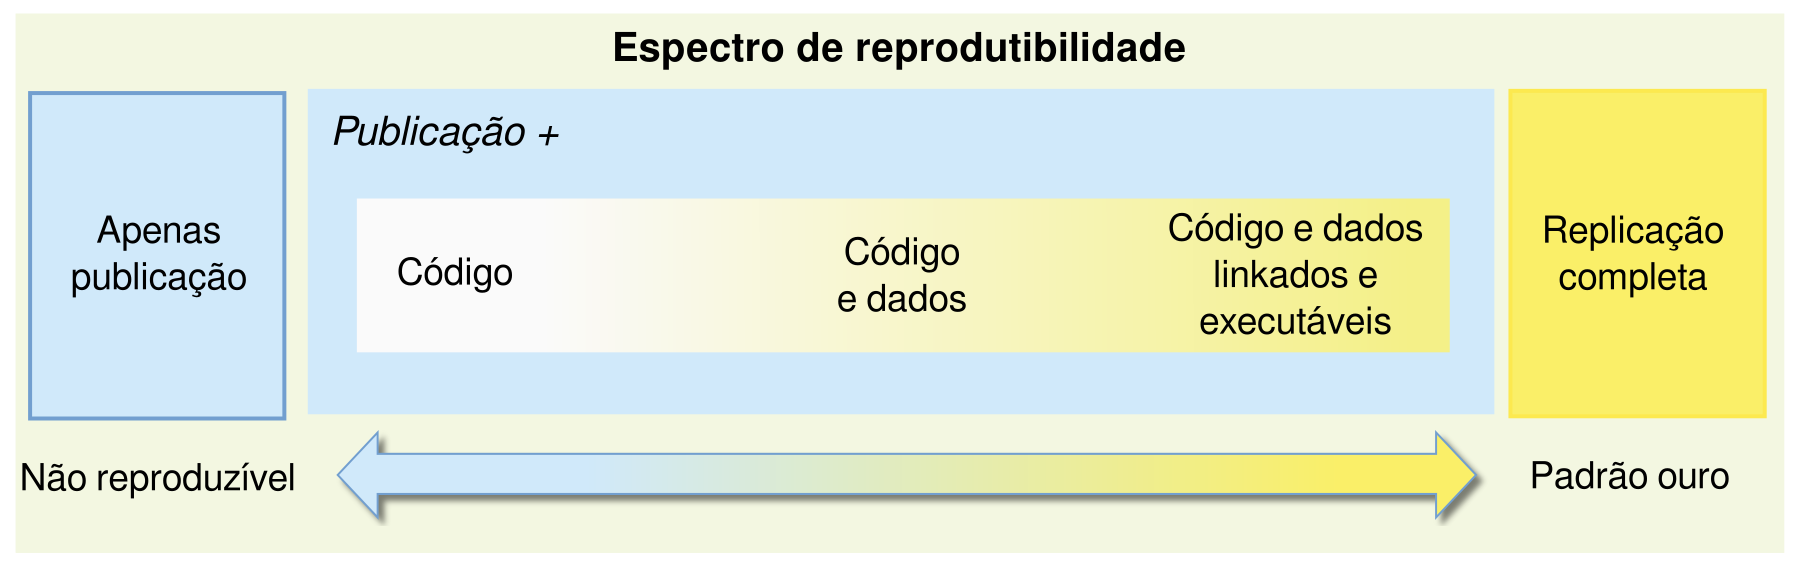
\includegraphics[scale=0.35]{imagens/reproducibility-spectrum-ptbr.png}
  \caption{Espectro de reprodutibilidade \cite{Peng2011}}
  \label{reproducibility-spectrum}
\end{figure}

Apesar das pesquisas reproduzíveis ({\it RR - Reproducible Research}) não
resolverem todos os problemas de validade experimental dos estudos em
engenharia de software, elas ao menos garantem que dados e métodos de análise
estejam disponíveis para inspeção e que os resultados possam ser derivados,
facilitando revisão logo que a publicação acontece. Além disso, é um recurso
valoroso para pesquisadores iniciantes, pesquisas reproduzíveis melhoram o
impacto do próprio estudo, por exemplo, artigos de computação que não
disponibilizam pubicamente dados e códigos possuem menos chances de serem
citados \cite{madeyski2017would}.

A disponibilidade dos softwares científicos tem sido enfatizada também em
discussões sobre sustentabilidade de software, um conceito que diz respeito
à longevidade dos sistemas de software.

%% O surgimento do conteito de engenharia de software baseada em envidências (EBSE
%% - {\it Evidence-Based Software Engineering }) surgiu em um trabalho seminal
%% apresentado em 2004 na {\it International Conference on Software Engineering
%% (ICSE)} e suas ideias e ferramentas, especialmente a revisão sistemática, tem
%% evoluído e amadurecido ao longo do tempo, e tem ajudado a caracterizar e
%% consolidar nosso conhecimento sobre muitos aspectos da pesquisa e práticas da
%% engenharia de software.
%% 
%% Em engenharia de software o termo {\it literatura} foi adicionado formando
%% revisão sistemática de literatura, isto foi feito para evitar confusão com
%% práticas de inspeção de código (comumente definido com o termo revisão) existentes
%% na área.
%% 
%% O objetivo de uma revisão sistemática é buscar e identificar todo material relevante
%% relacionado a um certo tópico (a natureza deste material é determinada pelas
%% questões de pesquisa e a natureza dos participantes intererssados na pesquisa).
%% 
%% Um fator em favor da aceitação dos conceitos da EBSE tem sido a crescente
%% reconhecimento que os resultados de estudos empíricos individuais são frequentemente
%% inconclusivos, e estes tipo de estudos são difícels de replicar com sucesso
%% \cite{sjoberg2005survey}.
%% 
%% Ainda existem poucos estudos replicados \cite{kitchenham2015evidence}.

\section{Sustentabilidade de software} \label{sustentabilidade}

% Software Sustainability: The Modern Tower of Babel

O {\it Dagstuhl Perspective Workshop} é um evento organizado por e para um
pequeno grupo de pesquisadores sêniores de renome internacional, realizado
anualmente na universidade de Dagstuhl\footnote{\url{http://www.dagstuhl.de}}
com o objetivo de refletir sobre o atual estado da ciência da computação.

Através de uma discussão intensiva com foco estratégico o workshop explora
tópicos novos e emergentes da ciência da computação produzindo manifestos que
capturam tendências e desenvolvimentos relacionados aos tópicos explorados.

Realizado desde 2011 o workshop tem explorado diversos tópicos da ciência da
computação, como computação e paleografia, tecnologia da informação como ponte
entre biologia e medicina, métodos de aprendizado de máquina para segurança de
computadores, análise de performance e visualização, entre outros tópicos. Em
sua mais recente edição, o {\it Dagstuhl Perspectives Workshop on ``Engineering
Academic Software''} \cite{allen2017engineering} examinou o estado atual dos
softwares científicos, identificou problemas comuns em seu desenvolvimento,
reconhecimento e sustentabilidade.

Uma das contribuições chave deste workshop é um manifesto contendo um roteiro
para o futuro da engenharia de software profissional e acadêmica, com foco em
instrumentos de suporte para pesquisas em software científico. O manifesto é
expresso em termos de ações ``promessas'' destinado a usuários e
desenvolvedores de softwares científicos, com passos concretos para melhorar o
ambiente em que os softwares são produzidos.

Os compromissos expressados neste manifesto são agrupados em três conceitos gerais:
(i) garantir que softwares científicos sejam {\it citados} apropriadamente;
(ii) promover a {\it carreira} do engenheiro de software desenvolvedor de software científico; e
(iii) medir a qualidade e sustentabilidade do software científico durante e após o seu {\it desenvolvimento}.

No terceiro compromisso, relacionado ao conceito {\it desenvolvimento}, o Dagstuhl Manifesto enfatiza a necessidade de medir a
qualidade e a sustentabilidade dos softwares científicos, e define
sustentabilidade de software como capacidade de perdurar, software sustentável
é aquele que continua a estar disponível no futuro, em novas plataformas e se
atende às novas necessidades \cite{allen2017engineering}.

% campos da engenharia de software, e apesar dos inúmeros entendimentos sobre o
% conceito \cite{venters2014software}, 

Essa definição de sustentabilidade de software é encontrada em mais detalhes no
{\it Karlskrona Manifesto} \cite{becker2014karlskrona}, um documento que alerta
sobre os impactos que os sistemas e a tecnologia da informação causam no futuro
do planeta, convida praticantes e pesquisadores de software a refletir sobre
o tema sustentabilidade na área da ciência da computação.

Sustentabilidade é um conceito guarda chuva composto de múltiplas dimensões, em
sua dimensão técnica, chamada sustentabilidade técnica, temos a preocupação com
a longevidade da informação, dos sistemas, e infraestrutura, e sua adequada
evolução frente as condições do ambiente em constante mudança. Software ocupa
um papel central nessa discussão, ele pode levar a crescentes consumo de
recurso, crescimento da desigualdade social, e influenciar no ganho ou perda de
auto-estima individual.

Se sustentabilidade não for levada em consideração em projetos de software, não
importa qual o domínio ou qual o propósito do software, perde-se a oportunidade
de causar mudanças positivas no planeta e na sociedade.

%Pesquisadores de
%software podem contribuir identificando questões de pesquisa em seu campo para
%ajudar a melhor entender sustentabilidade em projetos de software, Discutir com
%seus pares e pensar sobre como sustentabilidade impacta sua área de pesquisa.
%
%Assim, surge um conjunto de ações que podem ser tomadas pelos diferentes atores
%em direção à garantir sustentabilidade nos projetos de software, ações para
%praticantes de software, pesquisadores, associações profissionais, educadores,
%cientes e usuários.
% 
% 
% Em resumo os dois manifestos, Dagstuhl e Karlskrona, exprimem o conceito de
% sustentabilidade necessários para este estudo, mas é importante citar que
% algumas iniciativas e outros manifestos também estão preocupados com questões
% similares, dentre os quais podemos destacar:
% 
%A ciência aberta e comunidades de pesquisa em software tem sido bastante ativas
%em criar manifestos visando chamadas para ação. Estes manifestos chamam para melhorar
%os softwares e os metadados de bibliografia para citação persistente destes softwares.
%Outros tópicos endereçados nestes manifestos incluem ênfase no acesso ao código fonte.
%
%Agências de financiamento como o {\it US National Science Foundation} estão começando
%a reconhecer produtos de pesquisa como software assim como fazem com as publicações.
%Isto reconhece as contribuições ao softwares assim como primeiro produto de pesquisa.
%
%O {\it Journal of the American Statistical Association (JASA)} irá agora insistir na
%disponibilidade do código e dados durante a revisão dos manuscritos \cite{baker2016scientists}.
%% 
%% \begin{itemize}
%% 
%%   \item Science Code Manifesto \cite{barnes2013science}
%% 
%%     Foco em código fonte escrito especificamente para processar dados de
%%     publicações, afirma que ``todo código fonte escrito especificamente para
%%     processar dados de uma publicação deve estar disponível para os revisores e
%%     leitores do paper''.
%% 
%%   \item FORCE11 Software Citation principles \cite{smith2016software}\footnote{\url{https://www.force11.org/software-citation-principles}}
%% 
%%     Enfatiza persistencia e claridade e diz que ``Software deve ser considerado
%%     um produto legítimo de pesquisas e devem ser possível de serem citados''.
%% 
%%   \item Open Access Pledge \cite{holcombe2011openaccess}\footnote{\url{http://www.openaccesspledge.com}}
%% 
%%     Concentra-se em publicar softwares e papers em locais de {\it open access}.
%% 
%%   \item Open Science Peer Review Oath\footnote{\url{https://f1000research.com/articles/3-271/v2}}
%% 
%%     Concentra-se em potencializar os revisores para exigir acesso aberto aos
%%     softwares, práticas reprodutíveis e revisões transparentes.
%% 
%%   \item UK RSE \cite{ukrse2013}\footnote{\url{http://rse.ac.uk/who}}
%% 
%%     Conscientização sobre a importância e o papel do {\it Research Software
%%     Engineer} através de comunicação e suporta institucional.
%% 
%%   \item Reproducibility manifesto \cite{Barba2012}\footnote{\url{http://lorenabarba.com/gallery/reproducibility-pi-manifesto}}
%% 
%%     Inclui termos para fazer softwares reusáveis por outros. Foco em
%%     reprodutibilidade, deixando sustentabilidade de software fora de questão.
%% 
%%   \item The GeoScience paper of the future initiative \cite{OntoSoft2016}\footnote{\url{http://www.scientificpaperofthefuture.org/gpf/what-is-a-gpf}}
%% 
%%     Possui um conjunto de requerimentos para softwares serem incluidos em
%%     papers.  Focando mais no paper em sí do que no software.
%% 
%%   \item FAIR principles \cite{wilkinson2016fair}\footnote{\url{https://www.nature.com/articles/sdata201618}}
%% 
%%     Foco em dados de pesquisa. O objetivo é fazer eles serem encontráveis,
%%     acessíveis, interoperável e reusável. Estes princípios podem ser
%%     generalizados para aplicar aos softwares.
%% 
%% \end{itemize}

\section{Análise estática de código fonte} \label{analise-estatica}

A análise estática de código fonte é o primeiro passo para coletar informações
necessárias em diversas atividades de verificação, medição e melhoria da
qualidade de produtos de software \cite{Cruz2009, Kirkov2010}. Ela é
realizada com base no código fonte de um programa ou sistema de software, e a
partir daí descobre problemas e propriedades de sua qualidade estrutural
\cite{Chess2007}.

Ferramentas de análise estática estão disponíveis há décadas, em especial,
para programadores. A ferramenta Lint \cite{Johnson1978}, considerada a
primeira ferramenta de análise estática \cite{Gosain2015}, foi criada para
examinar programas escritos em linguagem C e aplicar regras de tipagem mais
estritas do que as regras dos próprios compiladores da linguagem.

%Neste trabalho o nosso interesse reside em compreender características de
%qualidade interna de ferramentas deste domínio de aplicação, do ponto
%de vista de desenvolvedores interessados em manter e evoluir tais ferramentas
%melhorando seus atributos de qualidade interna.
%
%A seção \ref{analise-estatica} apresenta uma definição geral da análise
%estática de código fonte, suas aplicações, sua anatomia, seus formatos de
%representação intermediária e técnicas mais comuns. 

Análise estática de código fonte tem como objetivo prover
informações acerca de um programa a partir do seu código fonte sem
necessidade de execução, e sem requerer qualquer outro artefato do programa
além do próprio código.

É um ramo que possui muitas das suas abordagens em comum com os estudos da
área de análise de programas ({\it program analysis}), especialmente na área de
compiladores, onde atua especialmente nas primeiras etapas do processo de compilação.

A análise estática de código fonte é considerada uma atividade meio com
objetivo de suportar uma variedade de tarefas comuns da engenharia de
software; muitas dessas tarefas são substancialmente úteis em atividades de
manutenção. \citeonline{Binkley2007} define uma lista dessas
atividades, incluindo:

\begin{multicols}{2}
  \begin{itemize}
    \item Análise de performance
    \item Compreensão de programas
    \item Desenvolvimento baseado em modelos
    \item Detecção de clones
    \item Evolução de software
    \item Garantia de qualidade
    \item Localizaçao de falhas
    \item Manutenção de software
    \item Recuperação arquitetural
    \item Testes
  \end{itemize}
\end{multicols}

Seja em qual atividade for, a análise estática possui importância,
pois ao ser capaz de extrair informações diretamente do
código fonte de um programa, pode auxiliar a responder perguntas necessárias
para as diversas atividades de desenvolvimento e evolução de software. Essa
importância se torna ainda mais aparente diante da ``lei'' da tendência para
execução \cite{Harman2010} que indica que todos os tipos de notação tem a
tendência de se tornar executáveis.

\subsection{Usos da análise estática de código fonte} \label{usos}

A análise de programas trata, de modo geral, da descoberta de problemas e
fatos sobre programas, ela pode ser realizada sem a necessidade de executar o
programa (análise estática) ou com informações provenientes de sua execução
(análise dinâmica).

A ideia de que programas de computador podem ser utilizados para analisar
código fonte de outros programas tem uma história de mais de 40 anos.  O
programa PFORT \cite{Ryder1974} foi projetado para localizar potenciais
problemas na portabilidade de código Fortran; em função da diversidade de
dialetos de Fortran, uma compilação sem erros não indicava que o programa
estava correto segundo os padrões da linguagem \cite{Wichmann1995}.

Desde então, ferramentas de análise estática de código fonte têm surgido para
os mais diversos fins -- muitas delas a partir das pesquisas e
desenvolvimentos da área de compiladores.  O {\it parser} utilizado nessas
ferramentas têm funcionalidades análogas aos analisadores usados em
compiladores \cite{Anderson2008}.

O uso de tais ferramentas tem se
tornado mais comum no ciclo de desenvolvimento de
software, sendo aplicadas em uma infinidade de atividades distintas visto que o
campo de aplicação destas ferramentas é bastante variado, cobrindo diferentes
objetivos. De acordo com \citeonline{Chess2007}, as atividades em que análise
estática de código fonte é empregada, destacam-se:

\begin{description}

  \item \textit{Verificação de tipos}. 
    A forma mais amplamente utilizada de análise estática, e uma das quais os
    programadores estão mais familiarizados, é a checagem de tipo.
    Previne que acidentalmente atribuam valores de forma incorreta a
    variáveis. Ainda, ao capturar erros em tempo de compilação, esta checagem
    de tipo previne erros em tempo de execução.

  \item \textit{Verificação de estilo}. 
    Os verificadores de estilo são um tipo de análise estática que aplicam regras
    de forma mais superficial do que os verificadores de tipo. São regras
    relacionadas a espaços em branco, nomes, funções depreciadas, comentários,
    estrutura do programa, entre outros. Os erros reportados por verificadores de
    estilo são aqueles que afetam a leitura e a manutenabilidade do
    código fonte, não indicando potenciais erros em tempo de execução como
    fariam os verificadores de tipo.

  \item \textit{Compreensão de programas}. 
    Ferramentas de compreensão de programa ajudam programadores a terem uma visão
    clara frente a grandes programas de computador, ou seja, programas com
    alto volume de código fonte. Ambientes de desenvolvimento integrados (IDE)
    geralmente incluem funcionalidade de compreensão, por exemplo, ``encontrar
    todos os usos de um certo método'' ou ``encontrar a declaração de uma
    variável global''. Análises mais avançadas chegam a incluir, por exemplo,
    refatoração automática. Estas ferramentas de compreensão também são úteis
    para programadores interessados em entender código fonte escrito por
    outros programadores.

  \item \textit{Verificação de programas}.
    Ferramentas de verificação de programa aceitam como entrada uma especificação
    e um conjunto de código fonte e tenta provar que o código está deacordo
    com a especificação. Quando a especificação é uma descrição completa de
    todo o programa, a ferramenta de verificação poderá realizar uma checagem
    de equivalência para garantir que o código fonte e a especificação
    combinam de forma exata. Programadores raramente têm acesso a uma
    especificação detalhada suficientemente para ser usada numa checagem de
    equivalência, o trabalho de criar esta especificação pode ser maior do que
    o trabalho de escrever o próprio código fonte do programa, desta forma
    este tipo de verificação formal raramente acontece.

  \item \textit{Localização de bugs}. 
    Um localizador de bugs está
    preocupado em apontar locais onde o programa, possivelmente, irá se
    comportar de forma inesperada. A maioria das ferramentas de localização de
    bugs são fáceis de usar porque costumam vir com um conjunto de regras
    ({\it bug idioms}) para descrição de padrões de código que indicam bugs.
    Algumas destas ferramentas costumam usar os mesmos algoritmos utilizados
    por ferramentas de verificação de propriedade.

  \item \textit{Avaliação de segurança}. 
    Ferramentas de análise estática para segurança usam as mesmas técnicas
    encontradas nas outras ferramentas, mas por ter um propósito diferente,
    identificar problemas de segurança, aplicam estas técnicas de forma diferente.
    As primeiras ferramentas de segurança (ITS4, RATS, Flawfinder) eram pouco mais
    do que um {\it ``grep''} melhorado; na maior parte, elas escaneavam o código
    procurando por funções como por exemplo {\it ``strcpy()''} que são
    facilmente usadas de forma inadequada e devem ser inspecionadas
    manualmente no processo de revisão de código fonte.

\end{description}

\subsection{Anatomia da análise de código fonte} \label{anatomia}

Ferramentas de análise estática de código fonte estão organizadas em partes ou
componentes, responsáveis por implementar três funções básicas: a) extração de dados, b) geração de representação
intermediária, e c) análise \cite{Cruz2009, Binkley2007}.

\begin{description}

  \item \textit{Extração de dados}.
    O processo de recuperar dados para futuro processamento ou armazenamento é
    chamado de extração de dados. 

    O primeiro componente da análise de código fonte é a extração de dados,
    responsável por ler o código fonte do programa e gerar uma ou mais
    representações intermediárias. Em essência, este componente converte a sintaxe
    de um programa em uma outra sintaxe abstrata e mais adequada para análise
    posterior.

  \item \textit{Representação intermediária}.
    Exportar os dados extraídos para uma representação intermediária é uma
    estratégia comum para facilitar análise e transformação de dados e
    possivelmente adição de metadados.

    Os dados obtidos na extração precisam ser representados em um formato mais
    abstrato. Esta é a responsabilidade do segundo componente da análise de
    código fonte: armazenar os dados coletados usando uma representação
    intermediária em formato mais adequado para análise automática, abstraindo
    aspectos particulares do programa e da linguagem de programação.

    Alguns tipos de representação intermediária têm sua origem na área de
    compiladores, entre os formatos mais comuns, destacam-se:

    \begin{multicols}{2}
      \begin{itemize}
        \item Árvore sintática abstrata
        \item Grafo de fluxo de controle
        \item Árvore sintática abstrata decorada
        \item Grafo de dependência de módulos
        \item Atribuição estática única
        \item Grafo de dependência de valores
      \end{itemize}
    \end{multicols}

    Estas representações podem ser utilizadas tanto na análise estática quanto
    na análise dinâmica. O uso de um ou outro formato depende do tipo de
    análise e seu propósito. Pode-se combinar diferentes tipos no sentido de
    enriquecer e estruturar a informação extraída.

  \item \textit{Análise}.
    Este componente é responsável por realizar inferências a partir dos dados
    representados internamente. O processo requer que as informações
    armazenadas estejam interconectadas e também interrelacionadas com
    conhecimento anterior. Esta análise pode gerar conhecimento quantitativo
    ou qualitativo, como, por exemplo, métricas de software ou mineração de
    dados, respectivamente. Técnicas de visualização podem ser usadas para
    apoiar este processo.

    Diversas técnicas foram desenvolvidas ao longo do tempo para realizar
    análise, algumas delas são brevemente descritas na seção \ref{tecnicas}.

\end{description}

\subsection{Formatos de representação intermediária} \label{formatos}

Essencialmente, um formato de representação intermediária é uma abstração precisa
das propriedades de um programa representado em um domínio menor. Os
compiladores normalmente constroem esta representação a fim de possuir um
modelo do programa sendo compilado, é comum que compiladores utilizem diversos
formatos durante o curso da compilação.

Em ferramentas de análise estática estes formatos são utilizados durante a
fase de análise para cumprir diversos objetivos, como por exemplo, calcular
métricas de código fonte. A métrica de complexidade ciclomática de McCabe
\cite{McCabe1976}, por exemplo, é definida com base no grafo de fluxo de controle ({\it Control Flow Graph - CFG}) do
programa com o seguinte cálculo $CC = e - n + 2p$. Onde: {\bf e} é o número de
arestas; {\bf n} é o número de nós; e {\bf p} é o número de componentes
fortemente conectados no grafo.

Assim, percebe-se que cada formato de representação intermediária pode ter fins
e objetivos bastante distintos, dentre os formatos mais comuns podemos destacar
\cite{Nielson2015, Stanier2013, Cruz2009, Ramalho1996}:

\begin{description}

  \item \textit{Árvore sintática abstrata}.
    A árvore sintática abstrata (AST - {\it Abstract Syntax Tree}) representa um
    programa tratando os elementos do código fonte como operadores e
    operandos organizados em nós numa árvore, este formato de representação é
    muito popular em tradutores {\it
    source-to-source}\footnote{http://en.wikipedia.org/wiki/Source-to-source\_compiler}.

  \item \textit{Grafo de fluxo de controle}.
    O grafo de fluxo de controle (CFG - {\it Control Flow Graph} ou {\it Call Graph}) é um grafo direcionado
    representando a estrutura de controle de um programa e sua sequência de
    instruções, onde as arestas mostram os possíveis caminhos de execução. Este
    formato é amplamente utilizado em métodos formais para otimização de
    código fonte.

  \item \textit{Grafo de fluxo de dados}.
    O grafo de fluxo de dados (DFG - {\it Data Flow Graph}) é também um grafo
    direcionado onde as arestas representam o fluxo de dados entre as
    operações do programa, este formato pode ser visto como um companheiro do
    grafo de fluxo de controle (CFG) e pode ser gerado ao longo de uma mesma
    análise.

  \item \textit{Árvore sintática abstrata decorada}.
    Árvore sintática abstrata decorada (DAST - {\it Decorated Abstract Syntax Tree}) é
    uma árvore sintática abstrata (AST) melhorada através de um processo de
    definiçao de atributos para os símbolos do programa de forma declarativa
    com uso de uma Gramática de
    Atributos\footnote{https://en.wikipedia.org/wiki/Attribute\_grammar}.

  \item \textit{Grafo de dependência de módulos}.
    O grafo de dependência de módulos (MDG - {\it Module Dependence Graph}) é um grafo
    onde os módulos são representados como nós e as arestas representam as
    relacões entre eles, indicando dependência entre os mesmos.

  \item \textit{Atribuição estática única}.
    Atribuição estática única (SSA - {\it Static Single Assignment}) pode ser vista
    como uma variação ou uma propriedade de outros formatos de representação
    intermediária, é um método que faz cada variável ser atribuída apenas uma única
    vez, facilitando a descoberta de informaçoes sobre os dados representados.

  \item \textit{Grafo de dependência de valores}.
    O grafo de dependência de valores (VDG - {\it Value Dependence Graph}) é uma
    variação que melhora (ao menos para algumas análises) os resultados
    obtidos a partir da atribuição estática única (SSA). Ele representa tanto
    o fluxo de controle quanto o fluxo de dados e assim simplifica a análise.

\end{description}

\subsection{Técnicas de análise} \label{tecnicas}

Inúmeras técnicas e métodos distintos podem ser utilizados pelas ferramentas
de análise estática, seja com o objetivo de verificação de tipos, localização
de bugs, compreensão de programas, avaliação de segurança, ou outra finalidade
qualquer. Segundo \citeonline{German2003, Li2010, Hofer2010} as técnicas e
métodos mais comumente encontrados nas ferramentas atuais são:

\begin{description}

  \item \textit{Análise léxica}.
    A análise léxica é responsável por quebrar o programa em pequenos fragmentos
    (ou {\it tokens}) e verificar se estes fragmentos são palavras válidas
    para uma dada linguagem. A análise léxica não leva em consideração a
    sintaxe do programa, sua semântica ou a interação entre módulos.

  \item \textit{Combinação de padrões de texto}.
    A combinação de padrões de texto ({\it Text-based Pattern Matching}) é a
    maneira mais simples e rápida de procurar vulnerabilidades num código
    fonte.

  \item \textit{Inferência de tipos}.
    A inferência de tipos ({\it Type inference}) refere-se a identificar o
    tipo de variáveis e funções e avaliar se o acesso a elas está em
    conformidade com as regras da linguagem. Linguagens de programação com
    sistema de tipagem incluem mecanismos deste tipo de análise.

  \item \textit{Análise de fluxo de dados}.
    A análise de fluxo de dados ({\it Data flow analysis}) resume-se a coletar
    informação semântica do código fonte do programa, e com métodos algébricos
    deduzir a definição e uso das variáveis em tempo de compilação. O objetivo
    é mostrar que nenhum caminho de execução do programa acessa uma variável
    sem definição ou atribuição prévia.

  \item \textit{Verificação de regra}.
    A verificação de regra ({\it Rule checking}) consiste em checar a segurança
    do programa através de um conjunto de regras pré-estabelecidas.

  \item \textit{Análise de restrição}.
    A análise de restrição ({\it Constraint analysis}) consiste em gerar
    e resolver restrições no processo de análise de um programa.

  \item \textit{Comparação caminho}.
    Comparação caminho ({\it Patch comparison}) inclui comparação de caminho de
    código fonte e de código-binário e é usada principalmente para encontrar
    brechas de vulnerabilidade já ``conhecidas'' e previamente divulgadas por
    fornecedores e praticantes da indústria de software.

  \item \textit{Execução simbólica}.
    A execução simbólica ({\it Symbolic execution}) é usada para representar
    as entradas de um programa através do uso de valores simbólicos ao invés
    de dados reais, produz expressões algébricas sobre a entrada dos símbolos
    do programa durante o processo de implementação e pode detectar
    possibilidade de erros.

  \item \textit{Interpretação abstrata}.
    Interpretação abstrata ({\it Abstract interpretation}) é uma descrição
    formal da análise do programa. Pelo fato de apenas controlar atributos de
    programa de preocupaçao dos usuários, a interpretação da análise semântica
    é similar ao seu significado semântico real.

  \item \textit{Prova de teoremas}.
    Prova de teoremas ({\it Theorem proving}) é baseada na análise semântica do
    programa. Converte o programa em fórmulas lógicas e então tenta provar que
    o programa é um teorema válido usando regras e axiomas.

  \item \textit{Verificação de modelo}.
    O processo de verificação de modelos ({\it Model checking}) primeiro constrói
    um modelo formal do programa tal como uma máquina de estados ou um grafo
    direcionado, então examina e compara o modelo para verificar se o sistema
    cumpre as características pré-definidas. Esta técnica requer a definição e
    descrição das propriedades que devem ser verificados por um pedaço de
    software.

  \item \textit{Verificação formal}.
    Verificação formal ({\it Formal Checking} ou {\it Compliance Analysis}) é o
    processo de provar de forma automatizada que o código do programa está
    correto em relação a uma especificação formal dos seus requisitos.

  \item \textit{Análise de fluxo da informação}.
    Análise de fluxo da informação ({\it Information Flow Analysis}) identifica
    como a execução de uma unidade de código cria dependência entre entradas e
    saídas.

  \item \textit{Verificação de sintaxe}.
    Verificação de sintaxe ({\it Syntax Checks}) tem o objetivo de encontrar
    violação de regras tais como expressões mal-formadas ou fora do padrão.

  \item \textit{Verificação de intervalo}.
    A análise de verificação de intervalo ({\it Range Checking}) tem o objetivo
    de verificar que os valores dos dados permanecem dentro de intervalos
    especificados, bem como manter a precisão especificada.

\end{description}

Diante a variedade e a constante evolução da área de análise estática
\citeonline{Novak2010} fez um estudo propondo uma taxonomia e um conjunto de
dimensões para caracterização de ferramentas de análise estática, mais detalhes
sobre essas dimensões e categorias serão exploradas no Capítulo
\ref{caracterizacao-ferramentas}, no qual apresentaremos uma caracterização de
softwares científicos estudados neste trabalho.

\section{Complexidade estrutural} \label{complexidade}

%% Métricas de software podem ser classificadas em métricas de processo, métricas
%% de projeto e métricas de produto.
%% 
%% Métricas de processo medem atributos relacionados ao ciclo de desenvolvimento
%% e manutenção de software. Métricas de projeto indicam se a execução do
%% processo está progredindo conforme planejado (por exemplo, relação entre o
%% tamanho do software entregue e o esforço total dispendido em seu
%% desenvolvimento).
%% 
%% Métricas de produto medem atributos de produtos e artefatos, como documentos,
%% diagramas, código fonte e arquivos binários. Neste trabalho,
%% apenas métricas de produto serão utilizadas.
%% 
%% Métricas de produto podem ser classificadas em internas (medem propriedades
%% visíveis apenas aos desenvolvedores) ou externas (medem propriedades visíveis
%% aos usuários) \cite{Mohamed1994}.
%% 
%% Neste trabalho, são utilizadas métricas de produto e, especificamente,
%% métricas de código fonte, que cobrem aspectos de tamanho, complexidade e
%% qualidade que podem ser medidos a partir do código fonte de um software.
%% 
%% Métricas de software tem um escopo bastante abrangente, e o termo está
%% associado com muitas atividades da engenharia de software: Medidade e modelos
%% para estimativa de custo e esforço, Coleção de dados, Modelos e medidas de
%% qualidade, Modelos de confiabilidade, Métricas de segurança, Métricas
%% estruturais e de complexidade, Avaliação de maturidade de capacidade,
%% Gerenciamento através de métricas, Avaliação de métodos e ferramentas.
%% 
%% \subsection{Métricas de código fonte} \label{metricas-de-codigo}
%% 
%% As propriedades visíveis aos desenvolvedores podem ser medidas através de
%% métricas de código fonte. A observação e o monitoramento de seus valores podem
%% indicar aspectos relevantes à manutenibilidade de um programa. Dentre as
%% inúmeras métricas de código fonte nosso interesse está em métricas que indicam
%% características relevantes à modularidade de um produto de software,
%% complexidade estrutural e custo de mudança.

%Structural and Complexity Metrics
%Desirable quality attributes like reliability and maintainability cannot be
%measured until some operational version of the code is available. Yet, we
%wish to be able to predict which parts of the software system are likely to be
%less reliable, more difficult to test, or require more maintenance than oth-
%ers, even before the system is complete. As a result, we measure structural
%attributes of representations of the software that are available in advance
%of (or without the need for) execution; then, we try to establish empiri-
%cally predictive theories to support quality assurance, quality control, and
%quality prediction. These representations include control flow graphs that
%usually model code and various unified modeling language (UML) dia-
%grams that model software designs and requirements. Structural metrics
%can involve the arrangement of program modules, for example, the use
%and properties of design patterns. These models and related metrics are
%described in Chapter 9.

Do ponto de vista de métricas, neste trabalho, estamos interessados, de fato, na métrica
de complexidade estrutural SC ({\it Structural Complexity}), uma medida da
complexidade de projetos de sistema de software proposta por
\citeonline{Darcy2005} como indicador da complexidade dos sistemas de software
em relação à sua estrutura interna e ao relacionamento entre os seus
componentes.

Complexidade é um tema bastante amplo, e para compreender onde os
sistemas de softwares se encaixam neste contexto precisamos definir brevemente
o que vem a ser sistemas complexos.

Sistemas complexos são sistemas no qual grandes redes de componentes sem
controle central dão origem a um comportamento
coletivo complexo, com processamento sofisticado de informação, e adaptação
através de aprendizado ou evolução \cite{Mitchell2009}. As seguintes
características são comuns a todos os sistemas complexos:

\begin{description}

  \item[Comportamento coletivo complexo.] Apesar de serem compostos por
  elementos bastante simples individualmente, sistemas complexos podem exibir
  comportamentos coletivos bastante sofisticados.

  \item[Troca de sinais e processamento de informação.] Em cada um destes
  sistemas, seus componentes individuais consomem e produzem informação entre
  si. Parte do comportamento do sistema envolve transformação dessa informação.

  \item[Adaptação.] Sistemas complexos adaptam-se a novas situações de forma a
  aumentar suas chances de sobrevivência diante de novas condições em seu
  ambiente.

\end{description}

Os sistemas complexos podem ser classificados como naturais ou artificiais, os
sistemas naturais são aqueles cuja constituição não tem participação humana, ao
contrário dos sistemas artificiais que são projetados por humanos, com
objetivos e funções previamente definidos \cite{Simon1996}. Neste sentido,
sistemas de software podem ser caracterizados como sistemas complexos
artificiais, pois exibem comportamento coletivo complexo, realizam trocas de
sinais e processamento de informação e passam por adaptação para se adequar a
mudanças em seu ambiente.

Sistemas de software são compostos por componentes, em geral, chamados de
módulos, que possuem tanto estado quanto comportamento próprios,
módulos individuais de um sistema de software são simples quando comparados com
o sistema como um todo. Módulos produzem informação para outros módulos
através de parâmetros em chamadas de sub-rotinas e consomem informação através
dos valores de retornos destas chamadas. O fluxo contínuo de novos requisitos e
de mudanças no ambiente operacional de sistemas de software força-os a se
manter em constante evolução em busca de “sobrevivência”.

Esta medida é, possivelmente, um indicativo de problemas na manutenibilidade de
sistemas de software, em especial sobre o esforço necessário para atividades de
manutenção \cite{Terceiro2012}. Ela está relacionada a como os módulos de um
programa estão organizados bem como à estrutura interna de cada módulo. Esta
métrica pode dar indícios importantes sobre características arquiteturais de um
programa de software e pode explicar seus atributos de qualidade interna.

%Modularity
%Modularity describes the logical partitioning of software into several parts, components, and modules.
%Software will be easy to understand and change when composed of independent modules.
%“A Software Maintainability Evaluation Methodology”, 1981
%\cite{kumar2012survey}

%Faz um experimento usando CBO LCOM e outras metricas como preditor de manutenabilidade...
%\cite{Dagpinar2003}

%A complexidade de um sistema de software pode ser de três tipos: a complexidade
%do problema, a complexidade procedural, e a complexidade do projeto do sistema.
%Esta última é o foco deste trabalho.
%A complexidade do problema está relacionada ao domínio do problema.
%A complexidade procedural está relacionada à estrutura lógica da programa, em es-
%pecial do seu comprimento, em termos de número de tokens, linhas de código fonte, ou
%estruturas de controle. Este último tipo é o que iremos estudar neste trabalho.
%
%Os sistemas complexos podem naturais ou artificiais, uma colônia de formigas
%por exemplo pode ser caracterizado como um sistema complexo natural, onde
%individualmente cada formiga se apresenta como criatura relativamente simples,
%com instintos básicos como procurar alimento, responder a estímulos químicos
%vindos de outras formigas, combater intrusos, etc. No entanto, quando
%observadas coletivamente em uma colônia, as formigas aparentam ser muito mais
%sofisticadas. Elas são capazes de se organizar em diferentes atividades, criar
%estruturas complexas dentro de seu formigueiro, e de encontrar o caminho mais
%curto para uma fonte de alimento.
%
%Os sistemas naturais são aqueles cuja constituição não tem participação humana.
%Sistemas artificiais são projetados por humanos, com objetivos e funções
%definidos.  Sistemas artificiais podem ou não serem projetados à imagem de um
%sistema natural, e durante a sua concepção eles são discutidos em termos tanto
%de suas características (o que eles são) como de necessidades que eles devem
%satisfazer (o que eles deveriam ser) \cite{Simon1996}.
%
%É importante ressaltar que esta caracterização de sistemas de software como
%sistemas complexos diz respeito à estrutura interna dos sistemas, ou seja, aos
%componentes que o constituem e ao relacionamento entre estes componentes. Não
%foram considerados outros aspectos importantes de sistemas complexos, como por
%exemplo o seu relacionamento com o ambiente externo.
%
%como uma combinação das métricas de acoplamento (CBO) e coesão (LCOM4), 
%
%Sistemas de software, no entanto, se
%diferenciam dos sistemas complexos naturais pelo fato de serem projetados;
%consequentemente, o seu processo evolucionário não é intrinsecamente parte do
%seu comportamento, mas fruto da ação consciente de seus desenvolvedores.
%
%\cite{Tegarden1995}
%
%"The implication of this result is that, when
%designing, implementing, and maintaining software to control complexity, both coupling and cohesion should be considered jointly,
%instead of independently" Darcy 2005
%
%Many studies have demonstrated a significant correlation between
%LOC and the cyclomatic number. The researchers usually suggest that
%this correlation proves that cyclomatic number increases with size; that
%is, larger code is more complex code. However, careful interpretation of
%the measures and their association reveals only that the number of deci-
%sions increases with code length, a far less profound conclusion. The cyclo-
%matic number may be just another size measure. Chapter 9 contains more
%detailed discussion of validation for the McCabe measures.
%
%{\bf SC} {\it Structural Complexity (Complexidade estrutural)}: mede a
%complexidade do software \cite{Darcy2005} combinando os valores de CBO e LCOM4.

\citeonline{Darcy2005} definem complexidade estrutural como uma combinação de
acoplamento e coesão. Estes são dois conceitos complementares: enquanto o
acoplamento reflete o relacionamento entre módulos, a coesão nos fornece uma
visão da organização dos componentes internos de um módulo e seus
relacionamentos.

Uma formalização da métrica proposta por \citeonline{Darcy2005} pode ser
expressa da seguinte maneira, para um projeto $p$ e seu conjunto de módulos
$M(p)$, a complexidade estrutural $SC(p)$ de $p$ é:

\begin{equation}
SC(p) = \frac
{ \displaystyle \sum_{m \in M(p)} CBO(m) \times LCOM4(m) }
{ |M(p)| }
\end{equation}

Esta medida de complexidade estrutural é portanto a complexidade
estrutural média entre todos os módulos do sistema.

\begin{itemize}

  \item {\bf CBO} {\it Coupling Between Objects (Acoplamento entre objetos)}:
    mede o acoplamento entre objetos do software \cite{Chidamber1994}
    calculando em nível de classe o número total de acessos à outras classes do
    mesmo sistema, é comum ser também chamada de Fan-out da classe. CBO é então
    definida pela seguinte fórmula:

\begin{equation}
\label{formula-cbo}
CBO(C) = \sum_{i=1}^{n} cliente(C, Ci)
\end{equation}

Onde:

\begin{equation}
cliente(Ci, Cj) =
  \begin{cases}
    1 \text{ se } Ci \Rightarrow Cj \wedge Ci \neq Cj \\
    0 \text{ caso contrario} \\
  \end{cases}
\end{equation}

A notação $ Ci \Rightarrow Cj $ indica acesso à atributos, variáveis, métodos ou funções
entre módulos ou classes.

Apesar de ser possível formalizar a métrica CBO através da fórmula acima, sua descriçao original é
bastante complexa, levando à implementações variadas do seu cálculo
\cite{Lincke2008}. A definição original, por exemplo, inclui explicitamente
acoplamento via herança \cite{Harrison1998}, no entando não deixa claro como
deve ser tratado métodos herdados \cite{Briand1999}. A definição original
afirma também que apenas chamadas explícitas (e não chamadas implicitas) de
construtores são contabilizadas. Algumas definições de CBO incluem não apenas $
cliente(Ci, Cj) $ mas também a recíproca $ cliente(Cj, Ci) $ de forma que o valor
final inclui classes que ela acessa somado ao número de classes do sistema que
a acessam \cite{Sant2008}.

Quanto mais as classes forem independentes, mais fácil é reutilizá-las e menos
arriscado é modificá-las. Classes mais acopladas precisam de mais rigor em
testes, pois mais partes do sistema dependem delas.

  \item {\bf LCOM4} {\it Lack of Cohesion in Methods (Ausência de coesão em
    métodos)}: mede o grau de falta de coesão em métodos \cite{Hitz1995}.

O cálculo de LCOM4 é dado através de grafo não-orientado em que os nós ou
vértices são os métodos e atributos de uma classe e as arestas são acessos à
métodos e atributos. O cálculo desta métrica pode ser formalizado como a
seguir \cite{Silva2012}.

Seja $ X $ uma classe qualquer e $ M_x $ o conjunto de métodos desta classe,
considere um grafo simples não-orientado $ G_x(V, E) $, sendo:

\begin{equation}
V = M_x
\text{ e }
E = \{ \langle m, n \rangle \in V \times V \}
\end{equation}

Onde:
\begin{equation}
(\exists i \in Ix : (m \text{ accessos } i) \land (n \text{ accessos } i)) \lor (m \text{ chamadas } n) \lor (n \text{ chamadas } m)
\end{equation}

O valor da métrica LCOM4 para uma classe $ X $ é então definido como o número
de componentes conectados do grafo $ G_x (1 \leq LCOM(x) \geq | M_x |)$.

Coesão entre os métodos de uma classe é uma propriedade desejável, portanto o
valor ideal para esta métrica é 1. Se uma classe tem diferentes conjuntos de
métodos não relacionados entre si, é um indício de que a classe deveria ser
refatorada em classes menores e mais coesas.

\end{itemize}
